% REVISÃO DA LITERATURA--------------------------------------------------------

\chapter{Revisão da Literatura}
\label{chap:revisao_da_literatura}

Para um melhor entendimento do presente trabalho, as Seções \ref{sec:esteganografia} a \ref{sec:stegdeeplearning} apresentam os principais conceitos de esteganografia, esteganálise e redes neurais (com foco em abordagens de aprendizagem profunda). Também serão apresentados os conceitos dos algoritmos de esteganálise e esteganografia relevantes para a avaliação dos resultados.
% avaliação dos resultados - em termos do que?

%------------------------------------------------------------------------

\section{Esteganografia}
\label{sec:esteganografia}

\definicoes{Esteganografia}
O principal objetivo da \textbf{esteganografia} é a transmissão de mensagens sem aparentar que uma comunicação secreta está em curso. Esse resultado pode ser obtido escondendo mensagens em objetos ordinários no canal de comunicação --- no meio digital objetos muito disseminados são imagens, áudios, vídeos e textos \cite{fridrich2009steganography}. Nesta seção serão apresentados conceitos básicos e as principais técnicas de esteganografia em imagens digitais.

\subsection{Conceitos}
\definicoes{Dado embutido, mídia de cobertura e estego objeto}
Em esteganografia, o conteúdo a ser escondido denomina-se \textit{embedded data} (\textbf{dado embutido}).
Essa mensagem será inserida em um objeto de cobertura qualquer, cuja denominação é \textit{cover object} (\textbf{mídia de cobertura}). A saída resultante da fusão dos dados embutidos com o objeto de cobertura é chamado de \textit{stego object} (\textbf{estego objeto}) \cite{petitcolas1999information}. O tipo da mídia de cobertura pode ser explicitado, utilizando-se, no caso de imagens digitais, os termos \textit{cover image} (\textbf{imagem de cobertura}) e \textit{stego image} (\textbf{estego imagem}).

\definicoes{Chave esteganográfica e sistema esteganográfico}
A chave, quando utilizada para esconder a mensagem, é denominada como \textit{stego key} (\textbf{chave esteganográfica}). Podemos definir o conjunto desses artefatos (dado embutido, mídia de cobertura, estego objeto e chave esteganográfica) como \textit{stegosystem} (\textbf{sistema esteganográfico} ou canal esteganográfico), cujo esquema está ilustrado na Figura~\ref{fig:stegosystem}.

\begin{figure}[!htb]
	\centering
	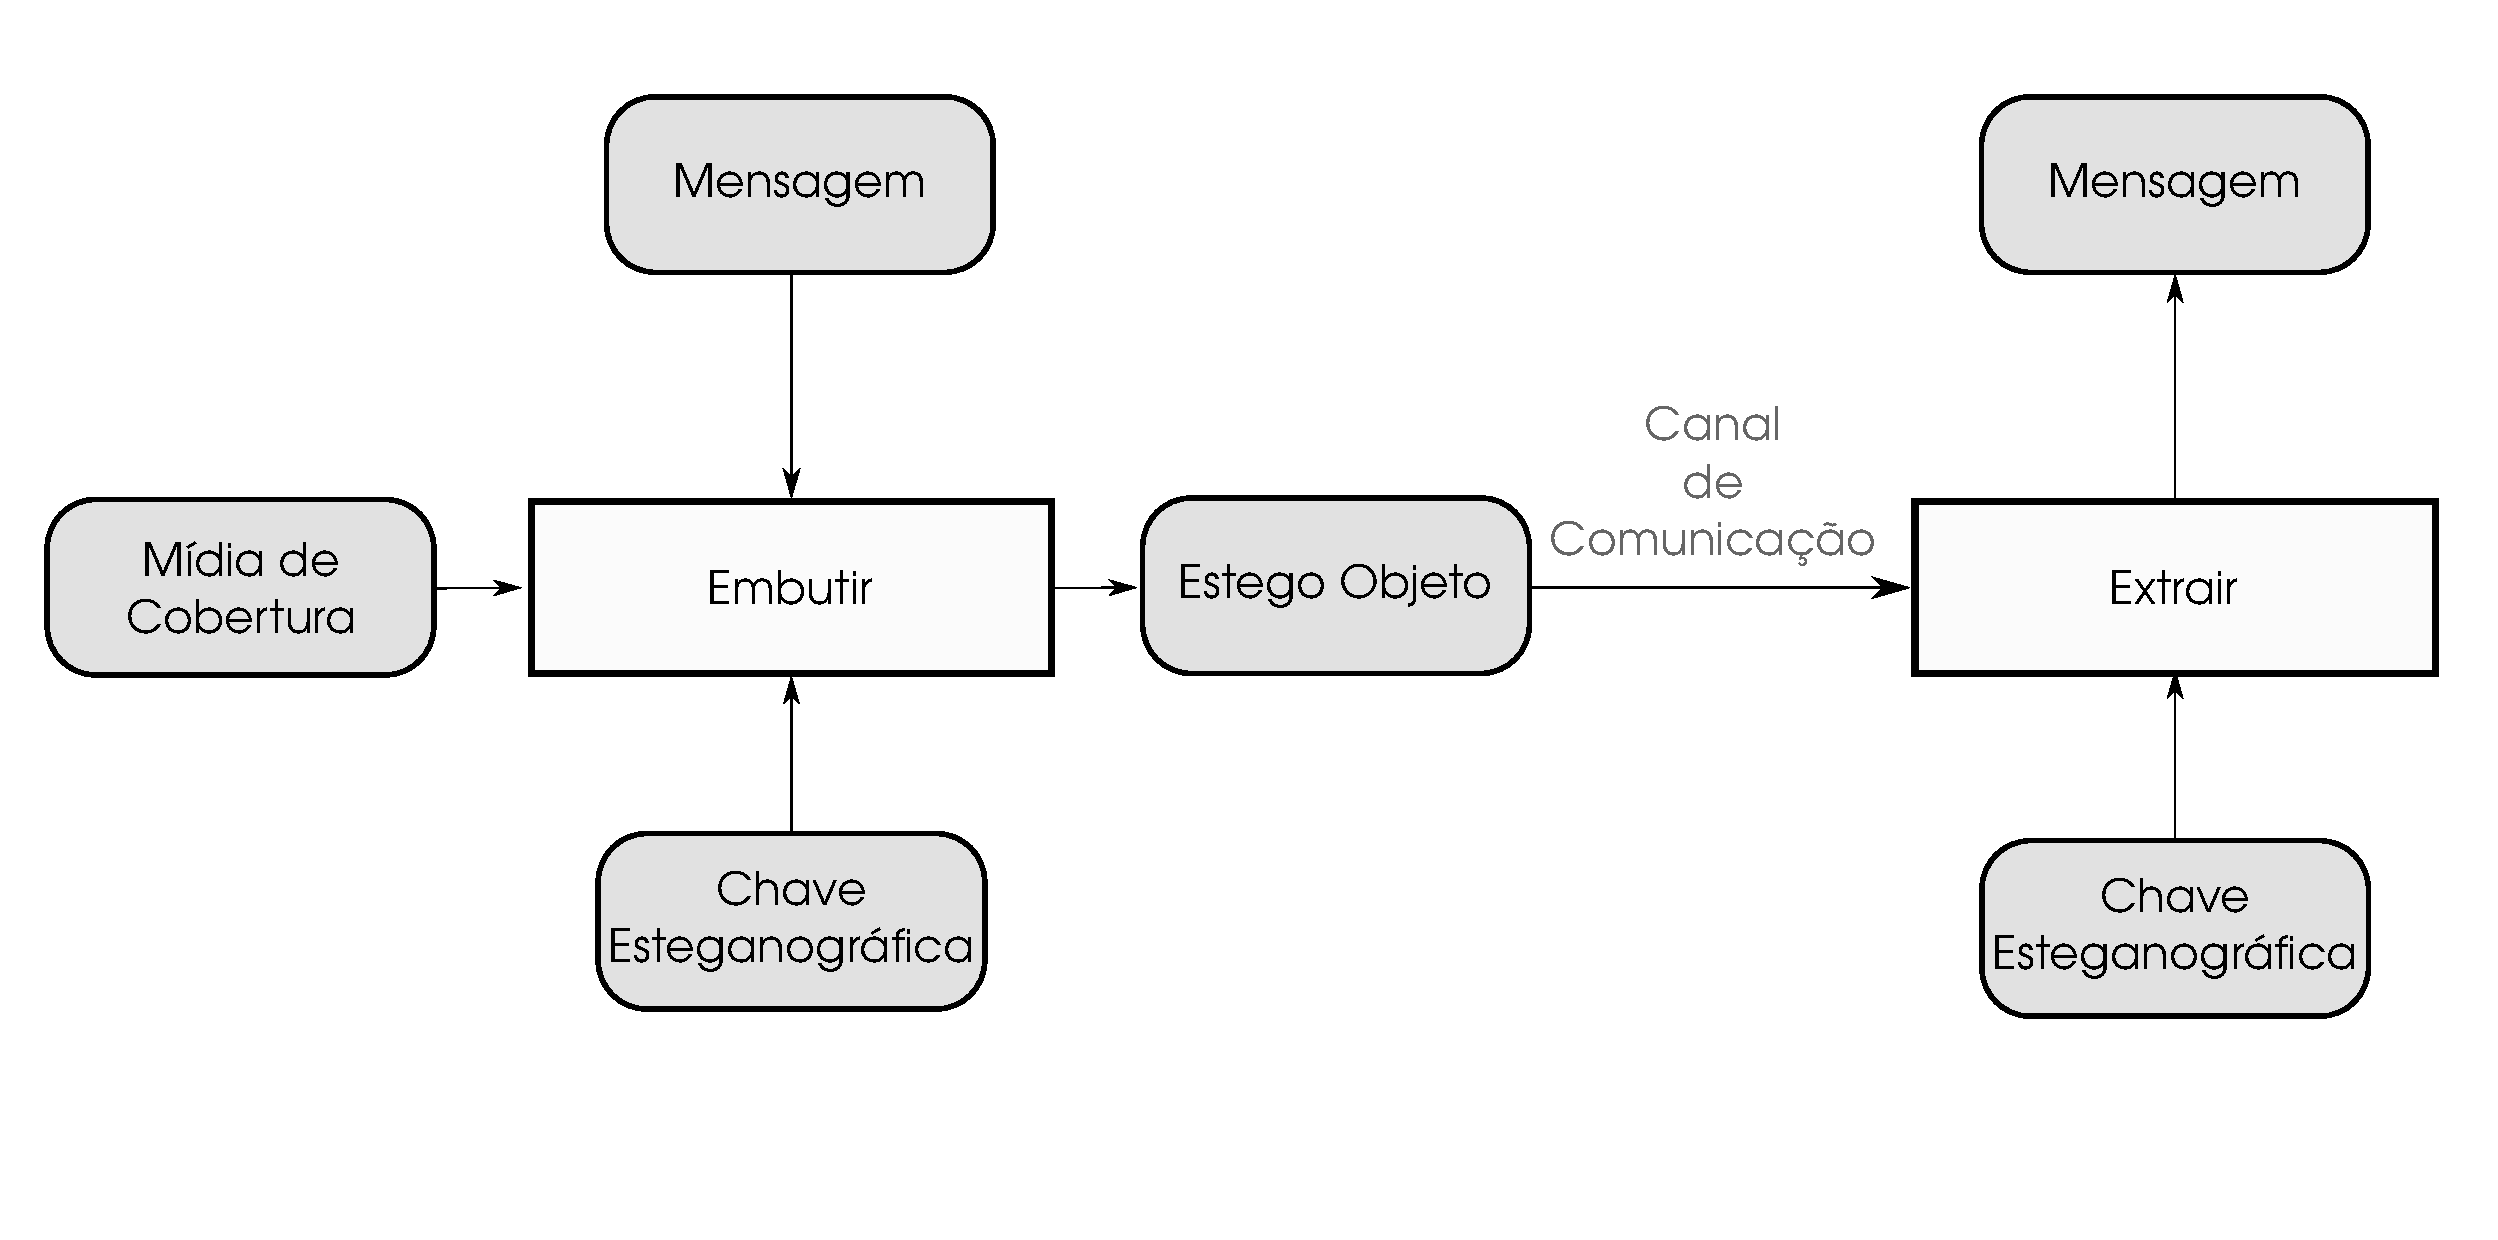
\includegraphics[width=1\textwidth]{dados/figuras/stegosystem.pdf}
	\caption{Elementos de um sistema esteganográfico (Autoria própria).}
	\label{fig:stegosystem}
\end{figure}

Quando a mídia de cobertura é uma imagem digital, a esteganografia pode atuar no \textbf{domínio espacial} ou no \textbf{domínio da frequência}~\cite{fridrich2009steganography}, sendo o primeiro o foco deste trabalho.

\definicoes{Domínio espacial}
No \textbf{domínio espacial} a imagem é representada por uma grade retangular densa de pixels,  %Essa abordagem é influenciada pelo método como imagens digitais são capturadas pelos sensores de câmeras digitais. 
gerando arquivos grandes e que permitem mensagens maiores embutidas~\cite{fridrich2009steganography}. No armazenamento utilizando mapa de bits, o qual será considerado nesse trabalho, a imagem é armazenada linha por linha, cada uma composta por pixels representados de acordo com o alcance de cores~\cite{cwayne1995graphicsfileformats}. Por exemplo, em imagens coloridas cada pixel é descrito por três bytes, em imagens em tons de cinza por um byte e em imagens binárias apenas um bit representa cada pixel.

\subsection{Métodos de Esteganografia}
\label{subsec:esteganografia-alg}

\definicoes{Não-adaptativos e adaptativos}
Há diferentes formas de escolher quais pixels da imagem de cobertura devem ser utilizados para esconder a mensagem. Esses métodos são divididos em \textbf{não-adaptativos} e \textbf{adaptativos}. Os métodos não-adaptativos não levam em consideração o conteúdo da imagem para escolher os pixels onde a mensagem será embutida, se baseiam na hipótese que os ruídos da imagem são independentes de pixel para pixel. Algoritmos \textbf{adaptativos} são os algoritmos que levam em consideração o conteúdo da imagem de cobertura para esconder a mensagem.

\definicoes{Sequencial e pseudo-aleatório}
Os principais métodos não-adaptativos para escolher os pixels da imagem são o \textbf{sequencial} e o \textbf{pseudo-aleatório}. O primeiro simplesmente esconde a mensagem sequencialmente na imagem, sendo que o primeiro pixel pode ser escolhido com base em um deslocamento arbitrário. O modo pseudo-aleatório utiliza a sequência de pixels definida por um gerador de números pseudo-aleatórios (PRNG, \textit{Pseudo-Random Number Generator}). A implementação desse método geralmente é feita derivando uma chave para um número inteiro que é utilizado como semente do PRNG. Por fim, no formato adaptativo, a escolha dos pixels depende do conteúdo da imagem de cobertura e é realizada por meio de heurísticas, as quais buscam minimizar a detecção.

\definicoes{Substituição e combinação} 
Após a seleção dos pixels, a inserção da mensagem na imagem é realizada por métodos que podem ser classificados como \textit{replacement} (\textbf{substituição}) ou \textit{matching} (\textbf{combinação}) \cite{ker}. Nos algoritmos por substituição, o bit menos significativo de cada um dos pixels selecionados é substituído pelo bit correspondente da mensagem. Algoritmos por combinação verificam se o bit da mensagem é o mesmo que o bit menos significativo do pixel. Se for igual, não é realizada nenhuma modificação. Caso contrário, aleatoriamente soma ou subtrai $1$ ao valor do pixel. Existem também alguns métodos diferentes de combinação propostos na literatura como, por exemplo, utilizar uma função que correlaciona dois pixels com o objetivo de realizar menores distorções na imagem~\cite{lsb_matching_revised}.

Sistemas adaptativos começaram a chamar a atenção através do princípio \textit{minimal impact embedding}. \textit{Minimal impact embedding}\definicoes{Modelo de imagem e codificador}são sistemas esteganográficos que separam seu design em \textbf{modelo de imagem} (\textit{image model}) e \textbf{codificador} (\textit{coder}) --- no que se refere ao modelo (e suas heurísticas) utilizado para escolher os pixels e a maneira que ele irá codificar a mensagens neles, respectivamente~\cite{fridrich2007steganography}. Os modos sequencial e pseudo-aleatório são modelos de imagem não-adaptativos e os métodos substituição e combinação são codificadores não-adaptativos. Os modelos de imagem adaptativos tentam modelar os custos de modificação de cada pixel da imagem e os codificadores tentam embutir a informação na imagem minimizando a função de distorção do modelo de imagem.

\definicoes{Payload}
O \textbf{\textit{payload}} $\alpha$ determina a razão entre mensagem embutida na imagem e pixels com custo menor que infinito de acordo com o modelo de imagem, ou seja, seja $m$ o número de bits de uma mensagem e $k$ o número de elementos com o custo de distorção $\delta < \infty$ no modelo da imagem, então $\alpha = m/k$~\cite{trelliscode}. Em relação aos algoritmos não-adaptativos, todos os custos de distorção são menores que infinito, então, o \textit{payload} pode ser interpretado como a proporção da imagem $0 \le p \le 1$ que será utilizada para esconder a mensagem, sendo medido em bits por pixel (bpp). Neste trabalho todos os algoritmos utilizam o parâmetro \textit{payload}.

Um sistema esteganográfico é dito \textit{perfeitamente seguro} se a distribuição de probabilidade da mídia de cobertura corresponde exatamente àquela do estego-objeto~\cite{cachin2004information}. Esse problema é de difícil resolução com mídias digitais reais (naturais) porque exige o conhecimento exato de tal distribuição da mídia de cobertura. Embora métodos denominados \textit{geração de mídia de cobertura}~\cite{anderson1996,adams2008,ryabko2009} proponham uma solução para o problema, eles acabam gerando objetos tendenciosos e com muitos artefatos, e que podem ser facilmente detectados. Na prática esse problema não é resolvido na sua forma ótima, sendo que as soluções mais utilizadas  buscam minimizar as perturbações da distribuição de probabilidade, na esperança de que sejam encobertas pelos ruídos naturais da mídia de cobertura.

\subsubsection{LSB e LSB \textit{Matching}}
\label{subsec:lsb}

\definicoes{LSB}
Os algoritmos baseados na abordagem \textit{\textbf{L}east \textbf{S}ignificant \textbf{B}its} (\textbf{LSB}) substituem os bits menos significativos de diversos pixels da imagem para embutir a mensagem, i.e., o LSB utiliza o codificador de substituição. A implementação mais trivial é utilizando o modelo de imagem sequencial não-adaptativo, mas o modelo pseudo-aleatório com uma chave esteganográfica também é utilizado.

Seja uma imagem em escala de cinza $I$ formada por $n$ pixels $p_1, p_2, \dots, p_n$, tal que cada pixel $p_i = (b_{_{i,1}}, b_{_{i,2}}, \dots, b_{_{i,8}})$ é representado por um byte, em que $b_{_{i,j}}$ é um bit mais significativo do que $b_{_{i, j+1}}$. Seja também uma mensagem, $M = \{m_1, m_2, \dots, m_k\}$, de tamanho $k \leq n$. A função de embutir do LSB sequencial pode ser definida como:

\begin{equation}
	LSB(I, M, l) \implies p_l = (b_{_{l,1}},b_{_{l,2}}, \dots, b_{_{l,7}}, m_{_l}),
\end{equation}

\noindent em que  $l$ é a posição do bit da mensagem que está sendo embutido. Exemplos do LSB são ilustrados na Figura~\ref{fig:lsb}.

\floatsetup[figure]{style=plain,subcapbesideposition=center}
\begin{figure}
	\centering
	\sidesubfloat[]{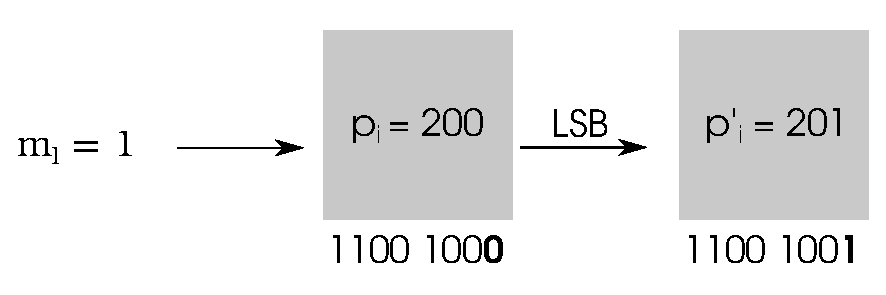
\includegraphics[width=0.75\textwidth]{dados/figuras/0-lsb.pdf}\label{fig:lsb-0}} \
	\sidesubfloat[]{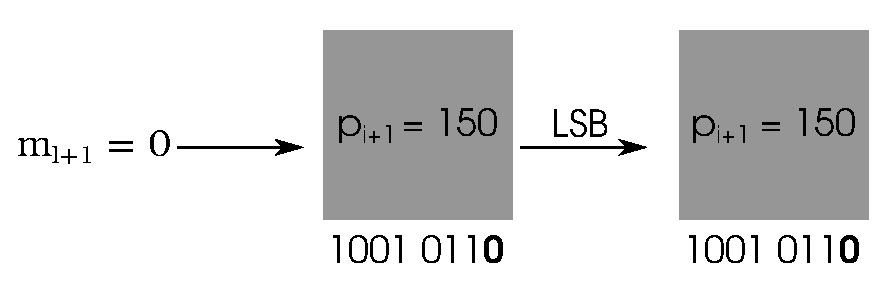
\includegraphics[width=0.75\textwidth]{dados/figuras/1-lsb.pdf}\label{fig:lsb-1}} \
	\sidesubfloat[]{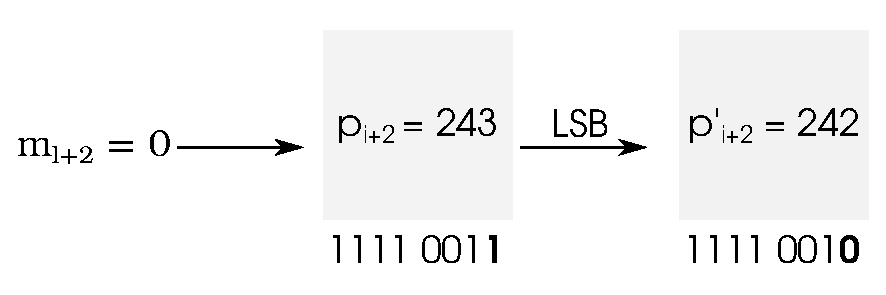
\includegraphics[width=0.75\textwidth]{dados/figuras/2-lsb.pdf}\label{fig:lsb-2}} \
	\caption{Codificação da mensagem $m = (1, 0, 0)$ nos pixels $p_i = 200$, $p_{i+1} = 150$ e $p_{i+2} = 243$. Em negrito está destacado o bit menos significativo de cada pixel. \protect\subref{fig:lsb-0} Representação da codificação do bit 1 no pixel $p_i$ com valor 200, resultando no pixel $p_{i+1}' = 201$; \protect\subref{fig:lsb-1} codificação do bit 0 da mensagem no pixel $p_{i+1} = 150$ não resultando em modificação; \protect\subref{fig:lsb-2} codificação do bit 0 no pixel $p_{i+2} = 243$ resultando no pixel $p_{i+2}' = 242$ (Autoria própria).}
	\label{fig:lsb}
\end{figure}

A abordagem LSB é muito empregada devido a sua simplicidade de implementação. Apesar disso, por atuar nos bits menos significativos, a modificação realizada é visualmente imperceptível~\cite{li2011survey}.

Desde 2004, o método de LSB por substituição se mostrou fraco a ataques estatísticos~\cite{ker} e resultados posteriores melhoraram sua detecção em algoritmos não-adaptativos~\cite{spam}.

\definicoes{LSB \textit{Matching}}
O \textbf{LSB \textit{Matching}}, como o próprio nome diz, utiliza o processo de \textit{matching} para esconder a mensagem, i.e., seu codificador é por combinação. Para ampliar sua segurança geralmente é utilizado o modelo de imagem pseudo-aleatório não-adaptativo para escolha da sequência de pixels a ser utilizada. Entretanto, também pode ser implementado utilizando a abordagem sequencial não-adaptativo.

Das várias abordagens existentes na literatura, a mais utilizada é a proposta por \citeonline{lsb_matching_revised}, conforme detalhada no Algoritmo~\ref{alg:lsb_matching_revised}. Ela permite que a mesma quantidade de dados seja escondida com menos modificações na imagem de cobertura.

Seja $M = \{m_1, m_2, \dots, m_k\}$ uma mensagem de tamanho $k$ a ser escondida e $Y = \{y_0, y_1, \dots, y_n\}$ a estego imagem. Para todo $m_i$ em que $i$ é par, $m_i = lsb(y_i)$, onde $lsb(x)$ retorna o bit menos significativo de $x$. Para todo $m_i$ onde $i$ é impar $m_i = f(y_{i-1}, y_i)$, em que $f(a, b)$ é uma função binária de correlação de $a$ e $b$. 

Considere as seguintes propriedades:

\newtheorem{property}{Propriedade}
\begin{property}
	$
		\label{eq:lsb_matching_f_property_0}
		f(l - 1, n) \ne f(l + 1, n), \quad \forall_{l, n} \in \mathbb{Z}
	$
\end{property}

\begin{property}
	$
		\label{eq:lsb_matching_f_property_1}
		f(l, n) \ne f(l, n + 1), \quad \forall_{l, n} \in \mathbb{Z}
	$
\end{property}

Caso elas sejam atendidas, é possível que o processo esteganográfico carregue uma informação a mais para o próximo pixel, resultando em menos modificações na imagem de cobertura. Um exemplo que atende estas propriedades é $f(a, b) = LSB(\lfloor a/2\rfloor + b)$. 

\begin{algorithm}
	\caption{LSB Matching}
	\label{alg:lsb_matching_revised}
	\KwIn{Um par de pixels $x_i, x_j$ da imagem de cobertura e dois bits $m_i, m_j$ da mensagem}
	\KwOut{Um par de pixels $y_i, y_j$ da estego imagem}
	\eIf { $m_i == lsb(x_i)$ } {
		\eIf { $m_j == f(m_i, m_j) $ }{
			$y_j \gets x_j$
		}{
			\tcc{Soma ou subtrai $x_j$}
			$y_j \gets \pm x_j$
		}
		$y_i \gets x_i$
	}{
		\eIf { $m_j == f(x_i - 1, x_j)$ }{
			$y_i \gets x_i - 1$
		}{
			$y_i \gets x_i + 1$
		}
		$y_j \gets x_j$
	}
\end{algorithm}


\subsubsection{HUGO}
\label{subsec:hugo}

\definicoes{HUGO}
\textit{\textbf{H}ighly \textbf{U}ndetectable Ste\textbf{go}} (\textbf{HUGO}) é um algoritmo para gerar um modelo de imagem adaptativo \textit{ad-hoc} para minimizar o impacto de detecção do descritor \textit{SPAM} (será visto com mais detalhes na Subseção \ref{subsec:spam}). Em implementações práticas, o HUGO é utilizado como modelo de imagem e o \textit{Syndrome-Trellis Code (STC)} \cite{trelliscode} como codificador. O algoritmo foi apresentado através de um novo modelo para definir custos de embutir através de descritores para esteganálise~\cite{hugo} (descritores para esteganálise podem ser vistos na Subseção \ref{subsec:esteganalise-alg}). Nesse modelo, os custos do HUGO são calculados a partir das matrizes de correlação do SPAM. A função de custo de embutir do HUGO é representada pela Equação~\ref{eq:distortion_function_hugo}:

\begin{equation}\label{eq:distortion_function_hugo}
	\begin{aligned}
		D(X, Y) = \displaystyle\sum_{d_1, d_2, d_3 = -T}^{T}
			\Bigg(
				&w(d_1, d_2, d_3) \left\lvert \displaystyle\sum_{k\in\{\rightarrow,\leftarrow,\uparrow,\downarrow\}}{} C_{d_1,d_2,d_3}^{X,k} - C_{d_1,d_2,d_3}^{Y,k} \right\rvert \\
			+	&w(d_1, d_2, d_3)\left\lvert \displaystyle\sum_{k\in\{\searrow, \nwarrow, \swarrow, \nearrow\}} C_{d_1, d_2, d_3}^{X, k} - C_{d_1,d_2,d_3}^{Y,k} \right\rvert
			\Bigg),
	\end{aligned}
\end{equation}

\noindent em que:
\begin{itemize}
	\item $T$ é um limiar entre 0 e 255;
	\item $X$ é a imagem de cobertura;
	\item $Y$ é a estego imagem;
	\item $C_{d_1,d_2,d_3}^{I,k}$ é a matriz de correlação da imagem $I$ na direção $k$;
	\item $w(d_1, d_2, d_3)$ é uma função de peso que tem a forma da Equação~\ref{eq:hugo_weight_function}.
\end{itemize}
\begin{equation}\label{eq:hugo_weight_function} w(d_1, d_2, d_3) = \frac{1}{\left(
					\sqrt{d_1^2 + d_2^2 + d_3^2} + \sigma
				\right)^\gamma},
\end{equation}

\noindent onde $\sigma, \gamma > 0$, são parâmetros que podem ser ajustados para minimizar a detecção.

O Algoritmo~\ref{alg:hugo} apresenta o pseudo-código do HUGO.

\begin{algorithm}
	\caption{HUGO \cite{hugo}}
	\label{alg:hugo}
	\KwIn{Todos os PIXELS da imagem de cobertura X}
	\KwOut{A estego imagem Y}

	\For { $(i, j)$ in $PIXELS$ } {

        \tcp{Calcula o impacto da codificação de +1}

		\algstat{stego\_plus \gets X.copy()}

		\algstat{stego\_plus[i][j]++}

		\algstat{embed\_impact\_plus[i][j] \gets D(X, stego\_plus)}

        \tcp{Calcula o impacto da codificação de -1}

		\algstat{stego\_minus \gets X.copy()}

		\algstat{stego\_minus[i][j]--}

		\algstat{embed\_impact\_minus[i][j] \gets D(X, stego\_minus)}
	}

	\tcp{Mínimo, elemento a elemento}

	\algstat{embed\_impact\_min \gets min(embed\_impact\_plus, embed\_impact\_minus)}

	\tcp{\textit{Syndrome Trellis-Code}}

	$\mathrm{pixels\_to\_change} \gets \mathrm{minimize\_embed\_impact}(LSB(X), \mathrm{embed\_impact\_min, message})$

	\algstat{Y \gets X}

	\eIf{ \algstat{model\_correction\_step\_enabled} } {
		\For { $(i, j)$ in $pixels\_to\_change$ } {
			\algstat{correction\_plus \gets Y}

			\algstat{correction\_plus[i][j]++}

			\algstat{dp \gets D(X, correction\_plus)}

			\algstat{correction\_minus \gets Y}

			\algstat{correction\_minus[i][j]--}

			\algstat{dm \gets D(X, correction\_minus)}

			\eIf{ $dp < dm$ }{
				$Y[i][j]++$
			}{
				$Y[i][j]--$
			}
		}
	}{
		\For { $(i, j)$ in $pixels\_to\_change$ } {
			\eIf{ $embed\_impact\_plus[i][j] < embed\_impact\_minus[i][j]$ }{
				$Y[i][j]++$
			}{
				$Y[i][j]--$
			}
		}
	}
	
\end{algorithm}


\subsubsection{S-UNIWARD}
\label{subsec:S-UNIWARD}

% a ideia é fazer as modificações onde o custo é mínimo

Historicamente, após bons resultados da função de distorção denominada \textit{Wavelet Obtained Weights} (WOW)~\cite{holub2012designing}, melhorias e generalizações no método deram origem uma função similar, o \textit{Uniward}~(\textit{Universal Wavelet Relative Distortion})~\cite{holub2014universal}. Ela representa a distorção na forma de uma soma de mudanças relativas entre a imagem de cobertura e a estego imagem representadas no domínio \textit{wavelet}.\definicoes{S-UNIWARD}Este trabalho abordará apenas o \textit{\textbf{S}patial \textbf{Uni}versal \textbf{Wa}velet \textbf{R}elative \textbf{D}istortion} (\textbf{\textit{S-UNIWARD}}), que trata da versão no domínio espacial da função \textit{Uniward}.

Em resumo, o S-UNIWARD é um algoritmo que gera um modelo de imagem adaptativo através de uma função de distorção para o domínio espacial, a qual calcula as mudanças relativas da estego imagem e da imagem de cobertura no domínio wavelet.

Na prática, após a utilização da função de distorção \textit{Uniward}, o esteganógrafo terá que utilizar uma função de codificação para minimizar a função de distorção. No domínio espacial geralmente é utilizado o STC (assim como no HUGO).

No \textit{S-UNIWARD}, a distorção depende da escolha de um banco de filtros direcionais e um parâmetro escalar para estabilizar os cálculos numéricos. Banco de filtros direcionais consiste em um conjunto de três filtros lineares, $\beta = \{K^{(1)}, K^{(2)},K^{(3)}\}$, invariantes a deslocamento~\cite{holub2014universal}. Esses kernels são utilizados basicamente para avaliar a suavidade da imagem nas direções horizontal, vertical e diagonal computando os resíduos direcionais $W^{(k)} = K^{(k)} \star X$, em que $W$ são os resíduos, $X$ é a imagem de cobertura e $\star$ é uma convolução \textit{mirror-padded}~\cite{holub2012designing}. Embora a direção dos filtros $K^{(1)}, K^{(2)},K^{(3)}$ podem ser escolhidos de forma arbitrária, \citeonline{holub2014universal} utilizaram kernels construídos a partir de filtros de decomposições \textit{wavelet} 1-dimensional passa-baixa $H$ e passa-alta $G$ da Equação~\ref{eq:filters}.

\begin{equation}
	\label{eq:filters}
	K^{(1)} = H \cdot G^T, K^{(2)} = G \cdot H^T, K^{(3)} = G \cdot G^T
\end{equation}

Seja $X$ e $Y$ um par de imagens de dimensão $n \times m$, e $W^{(k)}_{i,j}(X)$ e $W^{(k)}_{i,j}(Y)$ os $i,j$-ésimos coeficientes \textit{wavelet} correspondente as imagens $X$ e $Y$. A função de distorção \textit{Uniward} é definida pela Equação~\ref{eq:suniward}.

\begin{equation}
\label{eq:suniward}
	D(X, Y) \triangleq \sum_{k=1}^{3}\sum_{i=1}^{n}\sum_{j=1}^{m} \frac{|W_{i,j}^{(k)}(X) - W_{i,j}^{(k)}(Y)|}{\sigma + |W_{i,j}^{(k)}(X)|},
\end{equation}

\noindent sendo $\sigma > 0$ a constante de estabilização dos cálculos numéricos.


\subsubsection{MiPOD}
\label{subsec:mipod}

Historicamente, o design de sistemas esteganográficos para imagens digitais era muito dependente de heurísticas \textit{ad-hoc}. Essa abordagem deu origem a diversos métodos esteganográficos \cite{hugo,holub2012designing,holub2014universal,li2014new} que são realizados definindo uma função de custo para modificar cada pixel para, posteriormente, a mensagem ser escondida minimizando esse custo. Porém, todo esse paradigma é questionado, uma vez que não existe nenhuma conexão formal entre essas funções de distorção e a detecção estatística. É argumentado por~\citeonline{bohme2010advanced} que essa conexão pode nunca ser encontrada.

\definicoes{MiPOD}
O \textbf{MiPOD}, acrônimo para \textit{\textbf{Mi}nimizing the \textbf{P}ower of \textbf{O}ptimal \textbf{D}etector}, foi desenvolvido modelando a imagem de cobertura como um vetor $N$-dimensional, onde $X = \{x_1, x_2, \dots, x_n\}$ e cada $x_i$ é constituído através de uma distribuição gaussiana independente $x_i\sim\mathcal{N}(\mu_i, \omega_i^2)$ e quantizados em pontos discretos $k \in \mathbb{Z}$. Aqui, $\mu_i$ denota o conteúdo da imagem de cobertura sem ruído de captação, $\omega_i^2$ é a variância do ruído da captura. Nesse modelo, $z_i = x_i - \mu_i$ também é gerado por uma gaussiana independente $z_i \sim \mathcal{N}(0, \sigma_i^2)$.

Dada a imagem de cobertura $X = \{x_1, x_2, \dots, x_n\}$ a estego imagem $Y = \{y_1, y_2, \dots, y_n\}$ é obtida aplicando independentemente as seguintes regras de probabilidade:

\begin{align*}
	&\mathbb{P}(y_i = x_i + 1) = \beta_i, \\
	&\mathbb{P}(y_i = x_i - 1) = \beta_i, \\
	&\mathbb{P}(y_i = x_i)     = 1-2\beta_i,
\end{align*}

\noindent tal que $0 \le \beta \le 1/3$.

Com essas suposições sobre a imagem de cobertura e a estego imagem, é possível chegar em um detector ótimo que tem conhecimento de todas os desvios originais da imagem de cobertura $\sigma = (\sigma_1, \sigma_2, \dots, \sigma_n)$. Tal detector é representado pela Equação~\ref{eq:deteccao-otima}:

\begin{equation}
	\label{eq:deteccao-otima}
	\Phi = \sqrt{2\sum^N_{i=1}\sigma_i^{-4}\beta_i^2},
\end{equation}

\noindent que é o coeficiente de deflexão das duas hipóteses do detector (se é ou não uma estego imagem).

Para o estado da arte ser obtido, é preciso estimar a variância da imagem de cobertura para minimizar o poder de detecção da Equação~\ref{eq:deteccao-otima}~\cite{sedighi2016content}. O papel do esteganógrafo é, nesse caso, estimar a variância da imagem de cobertura; calcular a detectabilidade utilizando a Equação~\ref{eq:deteccao-otima}; criar o modelo de imagem adaptativo e os custos de codificar a mensagem. Uma ilustração desse modelo pode ser visto na Figura~\ref{fig:mipod}.

\begin{figure}[h]
	\center
	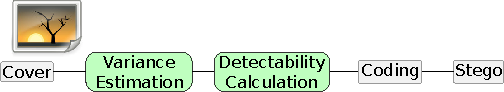
\includegraphics{dados/figuras/mipod.pdf}
	\caption{Etapas do MiPOD~\cite{sedighi2016content}.}
	\label{fig:mipod}
\end{figure}

%\subsubsection{Hill}
%\label{sec:hill}

\subsection{Comparação dos Métodos de Esteganografia}

% \begin{table}[h]
% 	\centering
% 	\begin{tabular}{| l | l |}
% 		\hline
% 		\textbf{Algoritmo}	& \textbf{Tipo} \\ \hline
% 		LSB			& Não-adaptativo \\ \hline
% 		LSB \textit{Matching}	& Não-adaptativo \\ \hline
% 		HUGO			& Adaptativo \\ \hline
% 		S-UNIWARD		& Adaptativo \\ \hline
% 		MiPOD			& Adaptativo \\ \hline
% 	\end{tabular}
% 	\caption{Abordagem dos algoritmos de esteganografia.}
% 	\label{tab:comp}
% \end{table}

Como discutido nas subseções anteriores, os algoritmos de esteganografia LSB e LSB \textit{Matching} são chamados de não-adaptativos pela aceitação da hipótese que os custos de embutir o \textit{payload} na imagem de cobertura são os mesmos independente do conteúdo da imagem. Por outro lado, os algoritmos HUGO, S-UNIWARD e MiPOD utilizam o princípio do \textit{Minimal Impact Embedding}, que separa o processo de esteganografia em modelo de imagem e codificador --- sendo o modelo de imagem os custos de se modificar cada pixel de acordo com o conteúdo da imagem de cobertura.

A Figura~\ref{fig:comp} ilustra o impacto dessa diferença de abordagem para a criação do modelo de imagem de cada algoritmo. Para uma mesma mensagem, é possível observar que os algoritmos adaptativos HUGO, S-UNIWARD e MiPOD modificam, respectivamente, 14,76\%, 12,69\% e 6,9\% da imagem, exemplificando o ganho de eficiência --- relacionado ao número de modificações --- entre os algoritmos adaptativos. Para os não adaptativos, a proporção da imagem alterada é consideravelmente maior.

\begin{figure}[h]
	\centering
	\subfloat[Imagem de cobertura]{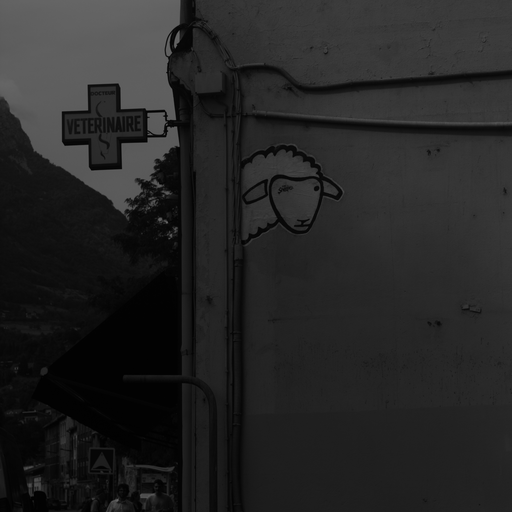
\includegraphics[width=0.25\textwidth]{dados/figuras/example-0-cover.png}\label{fig:cover}}\qquad
	\subfloat[LSB 25,65\%]{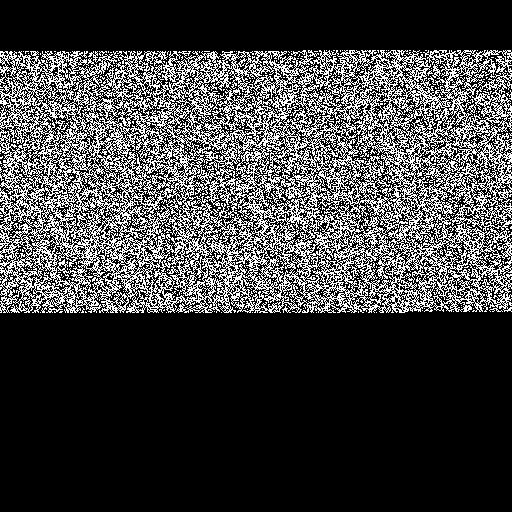
\includegraphics[width=0.25\textwidth]{dados/figuras/example-1-lsb.png}}\qquad
	\subfloat[LSB \textit{Matching} 14,6\%]{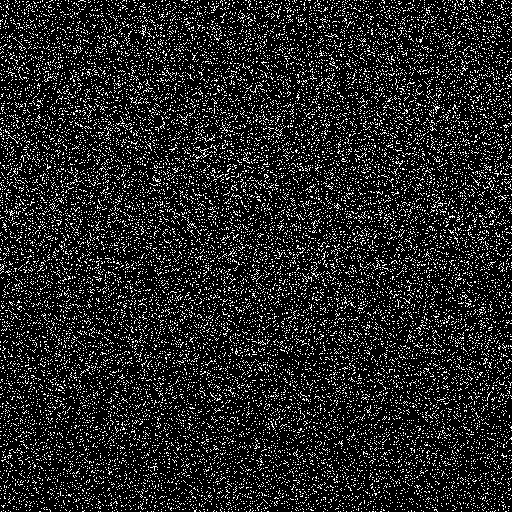
\includegraphics[width=0.25\textwidth]{dados/figuras/example-2-lsb-matching.png}}\qquad
	\subfloat[HUGO 14,75\%]{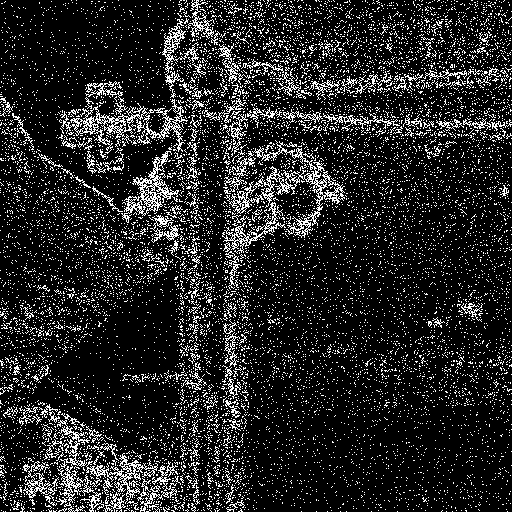
\includegraphics[width=0.25\textwidth]{dados/figuras/example-3-hugo.png}}\qquad
	\subfloat[S-UNIWARD 12,68\%]{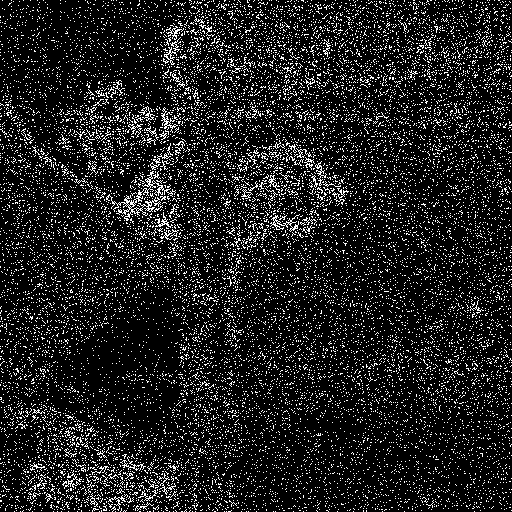
\includegraphics[width=0.25\textwidth]{dados/figuras/example-4-s_uniward.png}}\qquad
	\subfloat[MiPOD 6,9\%]{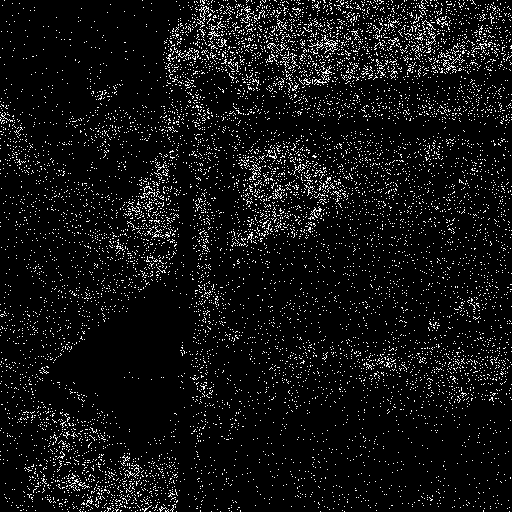
\includegraphics[width=0.25\textwidth]{dados/figuras/example-5-mipod.png}}\qquad
	\caption{Comparação das modificações feitas por diferentes algoritmos de esteganografia. \protect\subref{fig:cover} é a amostra 5008 da base BOSSBase~\cite{bas2011break}. As modificações estão representadas por imagens binárias, em branco as modificações realizadas para embutir um \textit{payload} de 0.6 bpp, em preto são os pixels não modificados de \protect\subref{fig:cover}. Ao lado do nome de cada algoritmo estão as porcentagens de modificação da imagem. (Autoria própria).}
	\label{fig:comp}
\end{figure}

Além disso, algumas características dos algoritmos podem ser observadas. Ao passo que o LSB inclui a mensagem de forma não-controlada, os algoritmos adaptativos buscam por regiões (tais como bordas) em que a alteração é menos perceptível.
%------------------------------------------------------------------------
\section{Esteganálise}
\label{sec:esteganálise}

O uso excessivo de algoritmos de esteganografia atrai estegoanalistas com o intuito de elaborar ataques para constatar a presença ou ausência de dados escondidos em imagens. Nesta seção, os métodos para atacar os algoritmos serão explicados mais detalhadamente.

\subsection{Conceitos}
\label{subsec:esteganalise-conc}

\definicoes{Esteganálise}
\textbf{Esteganálise} nada mais é do que o processo de detectar a esteganografia, ou seja, enquanto a esteganografia busca ocultar a existência informações, a esteganálise visa atacar essa forma de comunicação. Um estegoanalista tem sucesso em seu ataque caso consiga distinguir uma estego imagem de uma imagem de cobertura com probabilidade maior que o limiar de 50\% de acurácia, equivalente a um simples chute aleatório. Um ataque também pode ser planejado de modo a aproximar a quantidade de informação supostamente escondida na estego imagem \cite{fridrich2009steganography}.

\definicoes{Esteganálise cega e esteganálise direcionada} A esteganálise pode ser subdividida em duas classes principais: \textit{blind steganalysis} (\textbf{esteganálise cega}) e \textit{targeted steganalysis} (\textbf{esteganálise direcionada}). A primeira classe compreende os algoritmos de esteganálise que não levam em consideração o conhecimento prévio de um método de esteganografia específico, e a segunda consiste em planejar um ataque em um domínio de algoritmos pré-definido \cite{fridrich2009steganography}. Dado que o enfoque do trabalho é no domínio espacial, a seção terá foco na descrição dos algoritmos de esteganálise, cega e direcionada, no domínio espacial.


\subsection{Métodos de Esteganálise}
\label{subsec:esteganalise-alg}

\definicoes{Ataque visual}
A maneira mais simples de ataque esteganográfico é por meio aural, também chamado de \textbf{visual}. Esse ataque consiste em deslocar os bits menos significativos de cada pixel da imagem para as primeiras posições e preencher os demais com o mesmo valor. Dessa forma, os bits que menos influenciavam na imagem passam a ser os únicos relevantes. Por conseguinte, pixels que foram manipulados passam a divergir dos demais tornando visíveis rastros de informações escondidas \cite{wayner2009disappearing}. 

Um exemplo pode ser visto na Figura \ref{fig:visualattack}, onde a aplicação do ataque à imagem com uma mensagem oculta gerou, na parte superior, um comportamento discrepante em relação ao restante da imagem. Tal região corresponde aos pixels alterados pelo LSB.
\begin{figure}[ht]
\centering
	\subfloat[Imagem de cobertura]{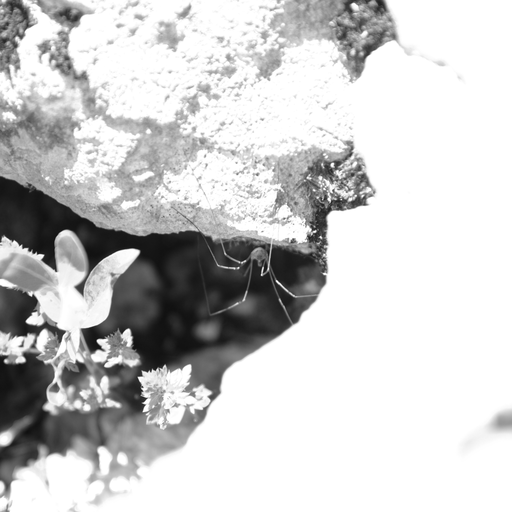
\includegraphics[width=0.25\textwidth]{dados/figuras/cover.png}}\qquad
	\subfloat[Ataque aural]{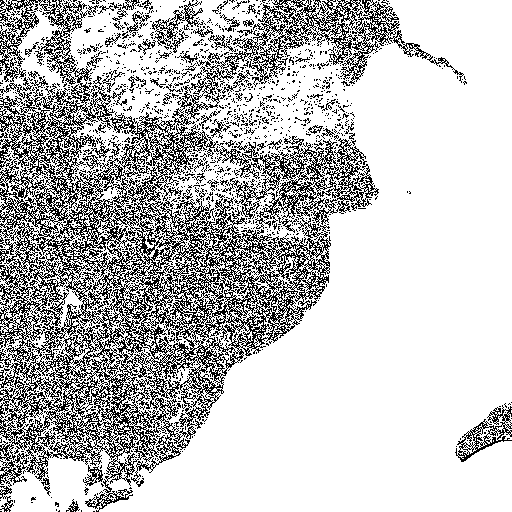
\includegraphics[width=0.25\textwidth]{dados/figuras/visual1.png}}\\ 
	\subfloat[Estego imagem]{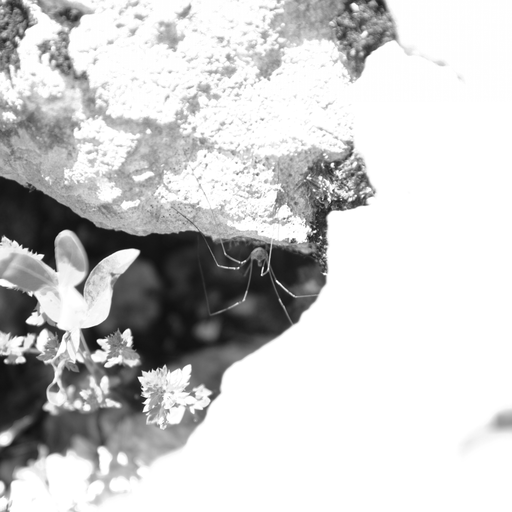
\includegraphics[width=0.25\textwidth]{dados/figuras/stego.png}}\qquad
	\subfloat[Ataque aural]{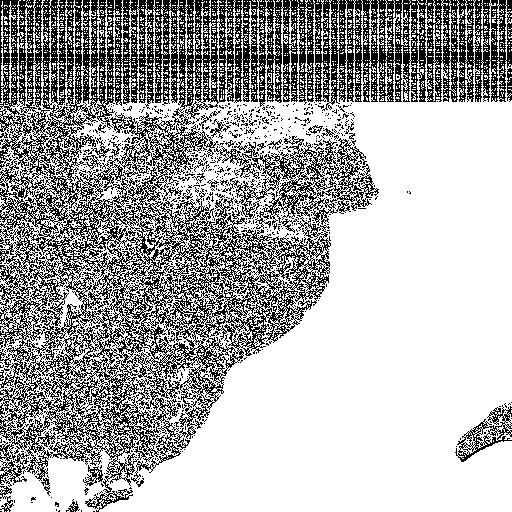
\includegraphics[width=0.25\textwidth]{dados/figuras/visual2.png}}

	\caption{Detecção do LSB por ataque visual. (a) Imagem 269 do BOSSBase~\cite{bas2011break}. (b) Ataque visual à imagem (a). (c) Estego imagem com LSB. (d) Ataque visual à estego imagem (Autoria própria).}
\label{fig:visualattack}
\end{figure}

\definicoes{Ataques estatísticos}
Verificar visualmente alterações na imagem tipicamente não é suficiente quando um método robusto de esteganografia é utilizado. Pode-se então aplicar \textbf{ataques estatísticos}, os quais analisam a distribuição dos pixels e seus bits menos significativos em uma imagem. Dessa forma, a partir de padrões frequentes, busca-se calcular a probabilidade de haver uma mensagem oculta na mesma \cite{fridrich2002practical}.

Esse tipo de ataque é muito empregado por depender somente da disposição dos bits na imagem. Nas seções subsequentes serão explicados os algoritmos estatísticos relevantes na área de esteganálise, bem como os que compõe o estado da arte atual. 

\subsubsection{Esteganálise sem Uso de Descritores}
\label{subsec:esteganalise-sem-descr}

O primeiro e mais simples método de esteganálise estatística, proposto por \citeonline{westfeld1999attacks}, é baseado no conceito de \textbf{par de valores} (POV, \textit{pair of values}), que são valores que diferem apenas no bit menos significativo. O ataque baseia-se na suposição de que, quando dados são escondidos em uma imagem, existe uma tendência à equalização dos valores de cada POV no histograma.

%Dada a intensidade de um pixel $c_{i} \in \{0, 1, \dots, 255\}$, podemos definir o i-ésimo POV como a tupla $(c_{2i}, c_{2i+1})$, resultando em 128 POVs diferentes. A estimativa da quantidade de informação escondida é obtida pelo teste $\chi^{2}$, o qual é definido pela seguinte equação:
%\begin{equation}
%	\label{eq:chi_square}
%	\chi^{2} = \sum\limits_{i=0}^{127} \frac{(n_{i} - n'_{i})^2}{n'_{i}},
%\end{equation}

%\noindent em que $n_{i}$ é o número de ocorrências do valor $c_{2i}$ em uma parcela imagem e $n'_{i}$ é metade da soma das ocorrências dos elementos do i-ésimo POV. A equação revela que, quanto maior a diferença do valor estimado para o encontrado, maior é a probabilidade da imagem conter dados escondidos. Em imagens onde os bits menos significativos são alterados de maneira sequencial, o algoritmo é bastante efetivo estimando, inclusive, a quantidade de informação escondida. Porém, como a técnica depende somente do histograma da imagem, é muito fácil contorná-la.

Devido às limitações da análise dos POVs, foi proposto por \citeonline{fridrich2002practical} um método de esteganálise mais robusto, denominado \textit{RS-Attack}. A sua ideia principal é avaliar a correlação espacial entre os pixels da estego imagem a partir de uma função discriminante. %calculada para um grupo $G = (x_{1}, x_{2}, \dots, x_{n})$ de pixels:
%\begin{equation}
%	\label{eq:rs_discriminant}
%	f(x_{1}, x_{2}, \dots, x_{n}) = \sum\limits_{i = 1}^{n-1} \abs{x_{i+1}-x_{i}}. 
%\end{equation}

%Quanto maior o valor dessa função, maior é o ruído encontrado no grupo $G$. Podemos ainda, definir uma função de \textit{flip} $F_{y}(x)$, na qual $y \in \{-1, 0, 1\}$ é a máscara aplicada, da seguinte maneira:
%\begin{equation}
%	\label{eq:flip}
%    \begin{cases}
%    	F_{1}(x), & 0 \leftrightarrow 1, 2 \leftrightarrow 3, \dots, 254 \leftrightarrow 255\\
%    	F_{0}(x), & x \\
%        F_{-1}(x), & F_{1}(x+1)-1 
%  	\end{cases}    
%\end{equation}

%Ao realizar operações sequenciais de \textit{flip} dos últimos bits do grupo com máscaras específicas, podemos gerar conjuntos $R$, $S$ e $U$ que condizem a, respectivamente: grupos em que as operações aumentam o valor de $f$, grupos em que as operações diminuem o valor de $f$ e grupos em que as operações não alteram o valor de $f$.

%A distribuição da quantidade de grupos nos conjuntos $R$ e $S$ revela características que permitem a estimativa do tamanho da mensagem escondida na imagem.

Contudo, o \textit{RS-Attack} tem um bom desempenho somente quando a esteganografia é feita com algoritmos muito simples, como o LSB. Com algoritmos como o LSB \textit{Matching} o desempenho é mediano.

Ambos os algoritmos são de implementação simples, mas apresentam complicações principalmente em imagens com grande quantidade de ruído, nas quais a quantidade de informação pressuposta pelo algoritmo para uma imagem de cobertura sem nenhuma informação é extremamente alta.\definicoes{\textit{Initial bias}}Esse fenômeno é denominado \textbf{\textit{initial bias}} e é tratado de maneira muito mais concisa quando se extrai características relevantes das imagens previamente.

\subsubsection{Descritor SPAM}
\label{subsec:spam}

Com o intuito de quebrar eficientemente
o LSB \textit{Matching}, uma análise empírica no banco de imagens BOWS2\footnote{http://bows2.gipsa-la.inpg.fr}
revelou que, em uma imagem natural, a probabilidade de pixels adjacentes terem valores parecidos é elevada. A representatividade dessa probabilidade pode ser vista na Figura \ref{fig:spam}, 
na qual a intensidade da escala de cinza é inversamente proporcional a probabilidade $Pr(I_{i,j} = x \wedge I_{i, j+1} = y)$ \cite{spam}.

\begin{figure}[!htb]
	\centering
	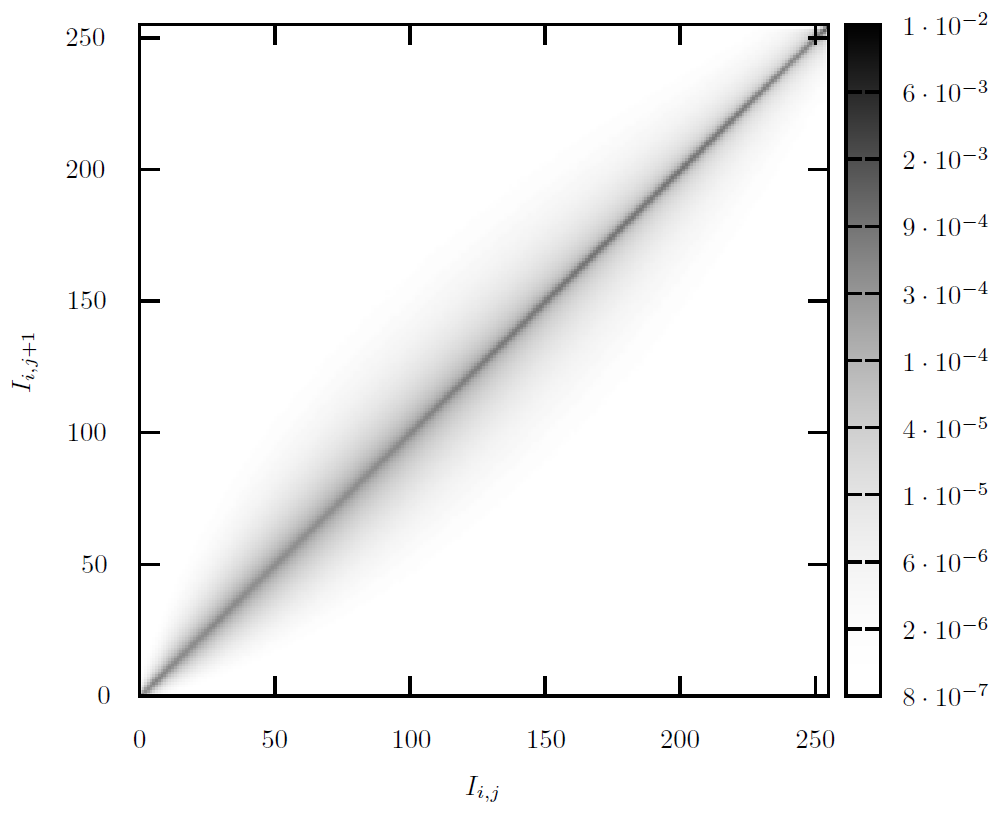
\includegraphics[width=.95\textwidth]{dados/figuras/SPAM1.png}
	\caption{Distribuição da probabilidade do valor de dois pixels horizontalmente adjacentes possuírem os valores descritos no eixo $x$ e $y$, em escala logarítmica \cite{spam}.}
    \label{fig:spam}
\end{figure}

Essa ideia abre a possibilidade de descrever a imagem a partir de uma matriz de probabilidades e selecionar estego imagens via um algoritmo de classificação. O primeiro método que utiliza uma matriz de probabilidades para a descrição de imagens é denominado \textit{\textbf{S}ubtractive \textbf{P}ixel \textbf{A}djacency \textbf{M}atrix} (\textbf{SPAM})\definicoes{SPAM} e se baseia nos gradientes direcionais da imagem de cobertura. A derivada direcional para a direita do pixel $I_{i,j}$, por exemplo, é dada pela Equação \ref{eq:derivada_direcional} e pode ser vista como um filtro linear espacial $[-1,1]$.

\begin{equation}
	\label{eq:derivada_direcional}
    D^{\rightarrow}_{i,j} = I_{i,j} - I_{i,j+1}
\end{equation}

O primeiro passo do algoritmo para gerar o descritor é computar as derivadas em todas as direções e sentidos possíveis: $\{\leftarrow, \rightarrow, \uparrow, \downarrow, \nearrow, \swarrow, \nwarrow, \searrow \}$, resultando em um vetor $\textbf{D}_{i,j}$ para cada gradiente possível. Para diminuir a dimensionalidade do descritor, o escopo é limitado a considerar somente os valores de $ \textbf{D}_{i,j} \in [-T, T]$, onde $T$ é um parâmetro passado previamente ao SPAM.

A matriz resultante é gerada a partir de uma cadeia de Markov \cite{lipschutz1998schaum}, podendo ser de primeira ou segunda ordem. Nas Equações \ref{eq:markov_1} e \ref{eq:markov_2}
 pode-se observar como cada posição $(u, v)$ e $(u, v, w)$ da matriz para a derivada à direita é gerada para ambas as ordens, respectivamente.
 
\begin{equation}
	\label{eq:markov_1}
    \textbf{M}^{\rightarrow}_{u,v} = Pr(\textbf{D}^{\rightarrow}_{i,j+1} = u | \textbf{D}^{\rightarrow}_{i,j} = v)
\end{equation}
 
\begin{equation}
	\label{eq:markov_2}
    \textbf{M}^{\rightarrow}_{u,v, w} = Pr(\textbf{D}^{\rightarrow}_{i,j+2} = u | \textbf{D}^{\rightarrow}_{i,j+1} = v |\textbf{D}^{\rightarrow}_{i,j} = w) 
\end{equation}
 
O descritor SPAM é a matriz de probabilidades resultante da cadeia de Markov. Um esquema que ilustra o processo do SPAM pode ser visto na Figura \ref{fig:spam2}.

\begin{figure}[!htb]
	\centering
    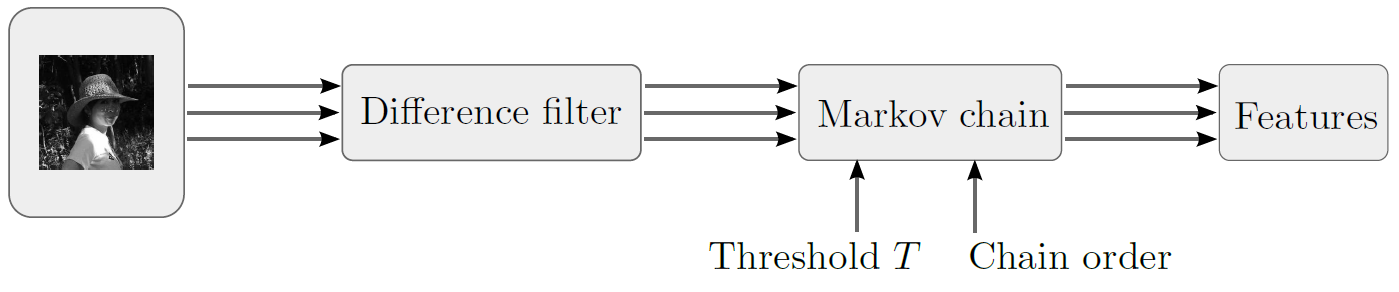
\includegraphics[width=.9\textwidth]{dados/figuras/SPAM2.png}
    \caption{Esquema de extração de características do SPAM \cite{spam}}
    \label{fig:spam2}
\end{figure}

A contribuição do SPAM na área de esteganálise é fundamental, dado que muitos algoritmos de esteganografia, como o HUGO, tentam minimizar custos diretamente relacionados ao filtro espacial do SPAM. Não somente isso, ele é a base do SRM, atual estado da arte que não utiliza técnicas de aprendizagem profunda.

\subsubsection{Descritor SRM}
\label{subsec:srm}

\definicoes{SRM}
Proposto inicialmente para detectar eficientemente o HUGO, a esteganálise baseada em \textit{\textbf{S}patial \textbf{R}ich \textbf{M}odels} (\textbf{SRM}) tem processo semelhante ao introduzido na Figura \ref{fig:spam2}, sendo que a maior mudança ocorre na parte da filtragem a partir do \textit{kernel} de gradiente simples \cite{fridrich2012rich}. Da mesma maneira que no SPAM, análises empíricas da correlação entre pixels próximos em uma imagem natural levaram ao uso  de 45 matrizes residuais para o cálculo dos descritores.

As matrizes de correlação podem ser observadas na Figura \ref{fig:srm}. Os \textit{kernels} do tipo \textit{spam} são filtros lineares simples, enquanto os \textit{kernels} do tipo \textit{minmax} são calculados a partir de operações de mínimo e máximo de múltiplos filtros lineares diferentes. O \textit{kernel} 1d, por exemplo, gera dois resíduos a partir das equações: $min\{I_{i-1, j} - I_{i,j} , I_{i,j-1} - I_{i,j}, I_{i+1} - I_{i,j}\}$ e $max\{I_{i-1, j} - I_{i,j}, I_{i,j-1} - I_{i,j}, I_{i+1} - I_{i,j}\}$.

\begin{figure}[!htb]
	\centering
    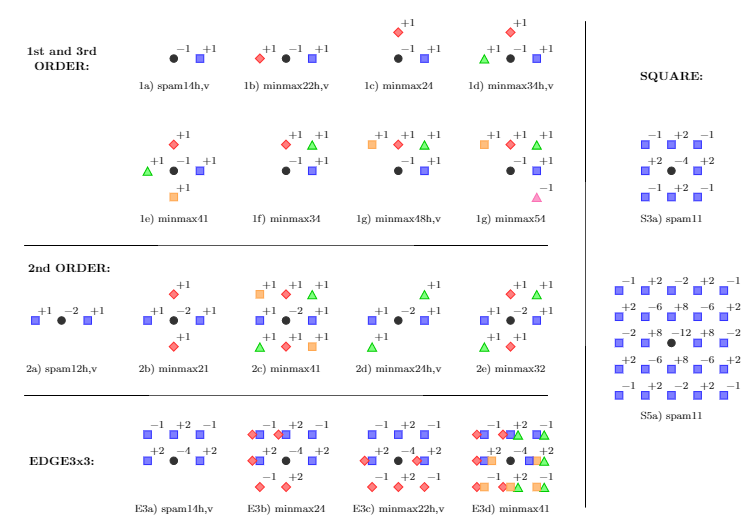
\includegraphics[width=\textwidth]{dados/figuras/kernels_srm.png}
    \caption{\textit{Kernels} de extração dos modelos SRM \cite{fridrich2012rich}}
    \label{fig:srm}
\end{figure}

Assim como no SPAM, são geradas as matrizes de correlação a partir de cadeias de Markov. O parâmetro $T$, no entanto, serve para truncar valores fora do intervalo $[-T, T]$, ao contrário de ignorar esses valores, como ocorria no SPAM.

O descritor SRM e suas variações se consolidaram na área de esteganálise como estado da arte até os modelos de redes de aprendizagem profunda. Apesar disso a classificação via \textit{Ensemble of Classifiers} e SRM ainda é muito utilizada devido a alta eficiência e o tempo reduzido de treino e teste com comparação métodos com aprendizagem profunda e é base para comparação de todos os algoritmos novos de esteganálise.


\subsubsection{Classificadores}
\label{subsec:classificadores}

Apesar da  possibilidade da classificação de uma imagem de cobertura ser realizada com qualquer classificador, o uso de um \textit{Ensemble of Classifiers} específico para esteganografia com SRM mostrou-se mais eficiente \cite{kodovsky2012ensemble}.

\definicoes{\textit{Ensemble of Classifiers}}
\textbf{\textit{Ensemble of Classifiers}} é a nomenclatura para o uso de diversos classificadores ao invés de somente um, chegando à classificação final a partir de um indicador formado pelo resultado individual de cada classificador (como uma votação, por exemplo).

Essa abordagem teve sua introdução e disseminação no âmbito esteganográfico devido ao baixo custo computacional aliado a bons resultados para um conjunto de características de alta dimensionalidade.

A escalabilidade com o número de amostras para treino sem perda de performance na classificação, se igualando a classificadores bem estabelecidos, como SVM, em conjunto com as outras características já listadas tornam o \textit{Ensemble of Classifiers} de FLDs ideal para o experimento proposto.%, no qual é aplicado um descritor de alta dimensionalidade (SRM) a uma grande quantidade de imagens para treino.


O modelo é composto pelo algoritmo de \textit{bootstrapping} para seleção de características e de imagens de treino e teste com classificadores do tipo \textit{Fisher Linear Discriminant} (FLD). 
 
A quantidade de classificadores e o tamanho da dimensão de características são definidos pelo algoritmo de otimização proposto por \citeonline{kodovsky2012ensemble}, que busca minimizar\definicoes{\textit{Out-of-bag error}}o \textbf{\textit{Out-of-bag error}} (OOBe), que é uma estimativa imparcial do erro de teste para \textit{Ensemble of Classifiers}. O valor do erro é calculado para cada sub classificador a partir da Equação \ref{eq:oob} \cite{fridrich2012rich}.
 
\begin{equation}
  \label{eq:oob}
    E^{(L)}_{OOB} = \frac{1}{2N^{trn}}\sum\limits_{m = 1}^{N^{trn}} (B^{(L)}(\boldsymbol{x^{(m)}}) + 1 - B^{(L)}(\boldsymbol{\bar{x}^{(m)}})),
\end{equation}

onde:

\begin{itemize}
\item $N^{trn}$ é o número de amostras definida para cada classificador.
\item $B^{(L)}(x)$ é o resultado da votação (imagem de cobertura = 0, estego imagem = 1) do classificador $L$ para o conjunto de características x.
\item $\boldsymbol{x^{(m)}}$ é o vetor de características da amostra de imagem de cobertura $m$ do conjunto de treino relativo a um classificador contendo imagens de cobertura sem informação escondida. 
\item $\boldsymbol{\bar{x}^{(m)}}$ é recíproco a $\boldsymbol{x^{(m)}}$, porém para o conjunto de estego imagens. 
\end{itemize}

%------------------------------------------------------------------------
\section{Redes Neurais}
\label{sec:redesneurais}

Partindo da hipótese que a atividade mental consiste de reações eletroquímicas de uma rede de células chamadas neurônios, alguns trabalhos pioneiros focaram em criar redes neurais artificiais, dando origem a área da inteligencia artificial chamada de \textit{conexionismo} ou \textit{computação neural}~\cite{russel}.

Um modelo matemático simples foi proposto em \citeonline{mcculloch-pitt} e pode ser visto na Figura~\ref{fig:neuron}. De forma simplificada, o modelo propõe um cálculo que realiza uma combinação linear das entradas conectadas e seus devidos pesos $w_{0,j}, w_{1,j}, \dots,w_{n,j}$. O neurônio é então ativado através de uma função de ativação baseada em um limiar.

\begin{figure}[!ht]
  \centering
  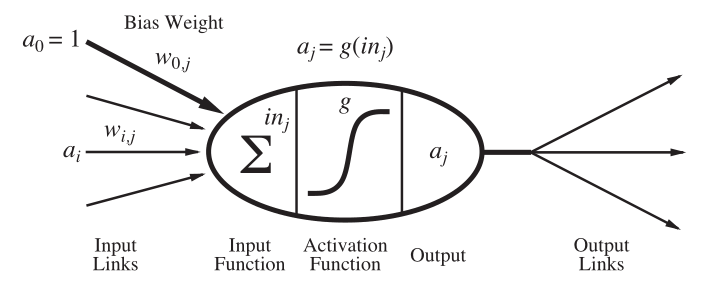
\includegraphics[width=0.85\textwidth]{dados/figuras/neuron.png}
  \caption{Modelo matemático proposto em \citeonline{mcculloch-pitt}, a imagem pode ser encontrada em \cite{russel}.}
  \label{fig:neuron}
\end{figure}

\definicoes{Rede neural}
Uma \textbf{rede neural} é simplesmente um conjunto de unidades neuronais conectadas, sendo que suas propriedades e funções são determinadas pela topologia ou pelas funções de combinação linear e ativação. %Como será abordado na Subseção~\ref{subsec:cnn}, uma rede neural baseada em funções de convoluções lineares em imagens chamada de \textit{Redes Neurais Convolucionais}. 

Na fase de treinamento de uma rede neural, cada entrada previamente rotulada é classificada pela rede e, caso a saída da rede seja diferente do esperado, os pesos das ligações entre os neurônios são reajustados a partir do vetor gradiente computado pelo algoritmo de aprendizagem. O gradiente indica se o erro iria aumentar ou diminuir caso o peso da ligação aumentasse levemente. O processo de reajuste dos pesos é denominado \textit{backpropagation}, pois se propaga entre as arestas de camadas cada vez mais superficiais até os neurônios iniciais da rede \cite{lecun2015deep}.

As funções de ativação abordadas neste trabalho são a tangente hiperbólica (TanH) e a unidade linear retificada (ReLU, \textit{rectified linear unit}), definidas pelas Equações \ref{eq:tanh} e  \ref{eq:relu}. 

\begin{equation}
	\label{eq:tanh}
    \text{TanH}(x) = \frac{1-e^{-\lambda x}}{1+e^{-\lambda x}}
\end{equation}

\begin{equation}
	\label{eq:relu}
    \text{ReLU}(x) = \text{max}(0, x)
\end{equation}


%\begin{equation}
%	\label{eq:softmax}
%    f(x)_i = \frac{e^{x_i}}{\sum_{j=1}^{K} e^{x_j}} \quad  \text{para }i = \{1, 2, ..., K\}
%\end{equation}

% \subsection{Conceitos}
\subsection{Aprendizagem Profunda}
\label{subsec:aprendizagemprofunda}

\definicoes{Aprendizagem profunda}
Uma rede de \textbf{aprendizagem profunda} (em inglês, \textit{Deep Learning}) é resumida estruturalmente como uma rede neural de diversas camadas intermediárias. Diversos trabalhos mostram que a sua performance é superior a métodos preliminares, fazendo com que estudos de redes neurais profundas sejam cada vez mais utilizados em diversas áreas do conhecimento~ \cite{lecun1990handwritten,lecun1998gradient,chen2015standard,lu2016wound,zhong2016field}.

Em um modelo tradicional de algoritmos de aprendizagem de máquina, o primeiro passo para a classificação é a extração de descritores condizentes com o problema, seguido da rotulagem do componente a partir de um classificador genérico. No caso da aprendizagem profunda as próprias camadas internas são responsáveis pela extração das características e pela classificação \cite{lecun1998gradient}.

A principal consequência da rede ser responsável pelo processo inteiro de classificação é a rede operar no modelo \textit{black box}, no qual há muito pouco controle sobre o seu treinamento. Quanto mais profunda é a camada, maior o nível de abstração dos dados e, consequentemente, menor é o controle sobre a respectiva etapa do processo.  

O modelo de arquitetura utilizado neste trabalho é o de Redes Neurais Convolucionais (CNN, \textit{Convolutional Neural Network}), o qual é muito empregado quando a entrada é uma matriz, como no caso de imagens digitais.

\subsection{\textit{Convolutional Neural Networks}}
\label{subsec:cnn}

\definicoes{CNN}
A principal diferença da \textbf{CNN} para uma rede neural convencional é o fato de que ela faz uso de camadas de convolução e subamostragem \cite{lecun2015deep}. As camadas de convolução são filtros lineares cujos \textit{kernels} tem os pesos ajustados no processo de \textit{backpropagation} e as camadas de subamostragem servem para reduzir a imagem para uma resolução menor. Normalmente o processo de subamostragem é realizado a partir de operações de \textit{maxpooling}, \textit{minpooling} e \textit{averagepooling}, que consistem respectivamente na seleção do maior, menor e média dos valores em uma janela de pixels. Um exemplo de \textit{averagepooling} pode ser visto na Figura~\ref{fig:average-pooling}.

A união dos subprocessos de modo a formar uma CNN completa pode ser vista na Figura \ref{fig:cnn}. 

\begin{figure}[!ht]
    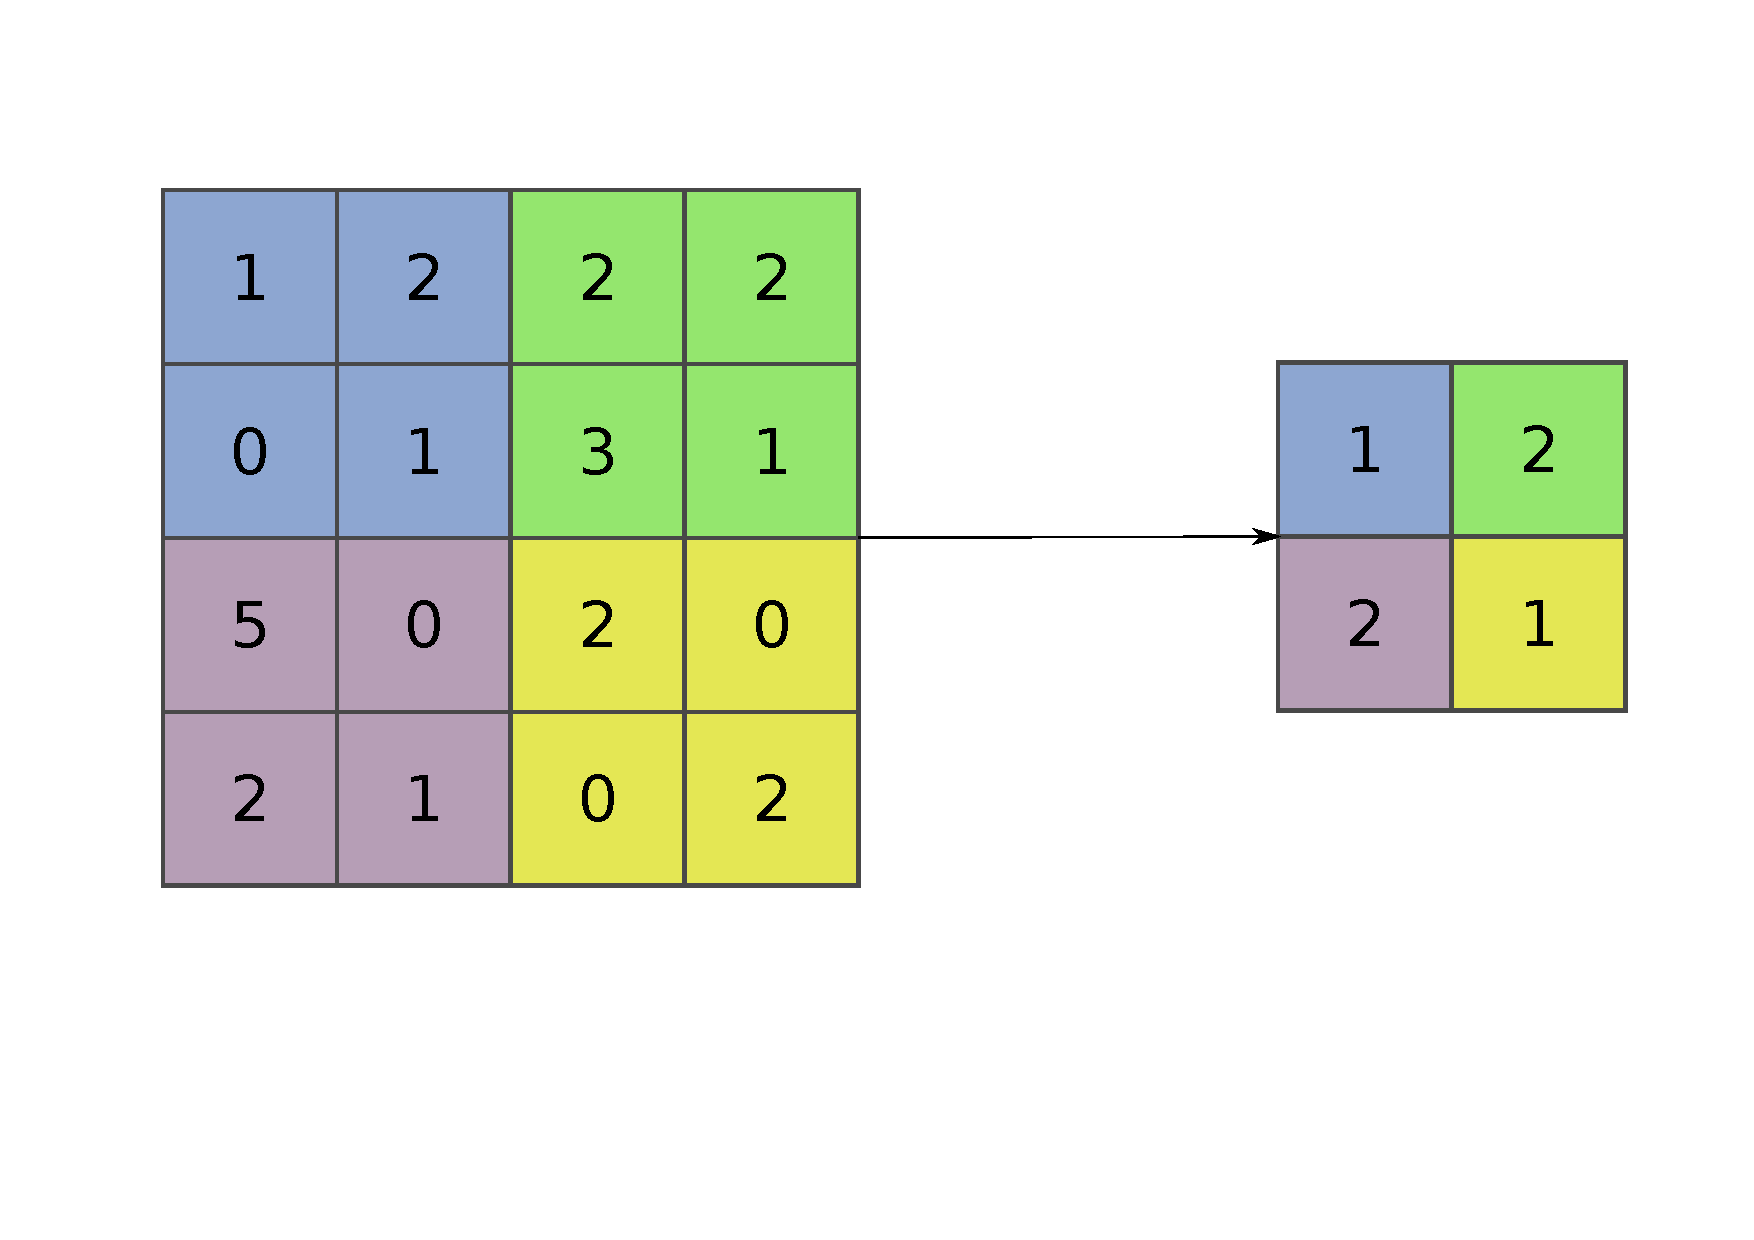
\includegraphics[width=\textwidth]{dados/figuras/average-pooling.pdf}
    \caption{Exemplo de \textit{averagepooling}, com uma janela de 2x2 e deslocamento (\textit{stride}) de 2, onde o a subamostragem é feita pela média dos valores em cada janela (Autoria própria).}
	\label{fig:average-pooling}
\end{figure}

\begin{figure}[!ht]
\centering
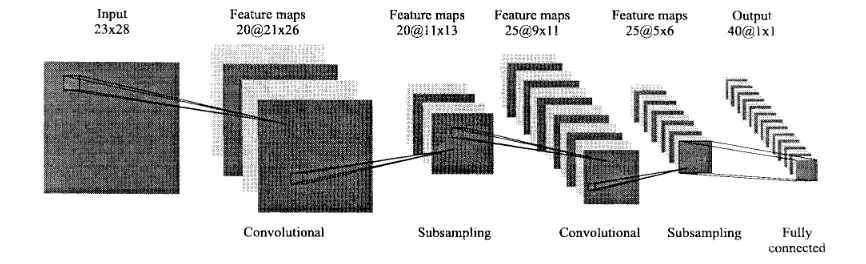
\includegraphics[width=0.95\textwidth]{dados/figuras/cnn.png}
\caption{Exemplo de uma CNN convencional \cite{lawrence1997face}.}
\label{fig:cnn}
\end{figure}

%------------------------------------------------------------------------
\section{Esteganálise via Aprendizagem Profunda}
\label{sec:stegdeeplearning}

Um modelo de esteganálise que faz uso de aprendizagem profunda independe do uso de qualquer descritor, logo todos os dados para treino e teste são as próprias imagens. A partir disso, a própria rede gera os descritores para a imagem e a classifica como imagem de cobertura ou estego imagem.

O uso de aprendizagem profunda para esteganálise é recente, sendo que o primeiro modelo utilizando CNN foi proposto em 2014 por \citeonline{tan2014stacked}, uma rede convolucional empilhada com \textit{auto-encoder} e os resultados foram significativamente inferiores ao SRM. Em 2015, \citeonline{qian2015deep} apresentaram resultados tão bons quanto os resultados do maxSRM (variação do SRM) com uma rede convolucional utilizando uma função ativação nova chamada de ativação gaussiana. \citeonline{cnn_base} desenvolveram uma arquitetura de CNN que incorpora um conhecimento do domínio da esteganálise, utilizando o \textit{kernel} do SPAM como pré-processamento. Na sequência, \citeonline{xu2016ensemble} propuseram um modelo de \textit{ensemble of CNN} que melhorou a acurácia do modelo anterior. O atual estado da arte provém de uma CNN residual extremamente complexa com 50 camadas de convolução~\cite{wu2017deep}. A rede errou em 4.9\% dos casos para o algoritmo MiPOD com \textit{payload} de 0.4 bpp, resultado muito acima de qualquer outro na área.
